\chapter{控制器仿真以及实际飞行实验结果分析}
\label{chap:simulatin_expermient}
本章之中,按照第\ref{chap:controller_design}
章中给出的控制器的数学模型,选定相应的初始条件进行双机的质点模型数学仿真:即不考虑无人机的姿态,只考虑无人机的位置,速度大小以及方向。之后,利用第\ref{chap:hardware}章中介绍的$ROS/Gazebo-PX4$仿真环境,在考虑无人机动力学的条件下进行双机编队仿真。
\section{基于MATLAB/Simulink的双机编队数学仿真}
本节数学仿真只验证编队控制器的控制性能以及控制逻辑的正确性,因而在仿真之前,做如下假设:
\begin{enumerate}
\item 无人机自动驾驶仪内环仅为一个具有时间常数$\tau$一阶惯性环节。
\item 无人机的姿态动力学没有过渡过程,即姿态动力学方程由相应的稳态方程代替。
\end{enumerate}
另外,按照第\ref{chap:controller_design}章中控制器设计分为水平平面以及竖直平面的原则,本节之中的仿真也是分为两个方面进行的;在任何
在其中任意一个平面内仿真时,都假设另外一个平面已经达到了控制目标,并且处于稳态。

在水平面的仿真中:选取的初始条件均为在地面坐标系$NED$中定义:
领机初始位置$P_{0}^{l}=(0,100)$;
领机初始速度$V_{0}^{l}=(20,0)$;
从机的初始位置$P_{0}^{f}=(0,0)$;
从机的初始速度$V_{0}^{f}=(10,10)$;
仿真的结果如下三图所示:其中,图\ref{fig:c5-matlab-pos},表示双机编队位置关系,横轴为NED坐标系下的E轴,纵轴为N轴。
图\ref{fig:c5-matlab-vel}以及图\ref{fig:c5-matlab-eta}分别表示双机速度大小以及速度方向的与时间的关系图。由仿真结果可得,
在算法层面上,第\ref{chap:controller_design}所设计的编队控制器在水平平面内可以完成编队控制的任务。
\begin{figure}[H]
    \centering
    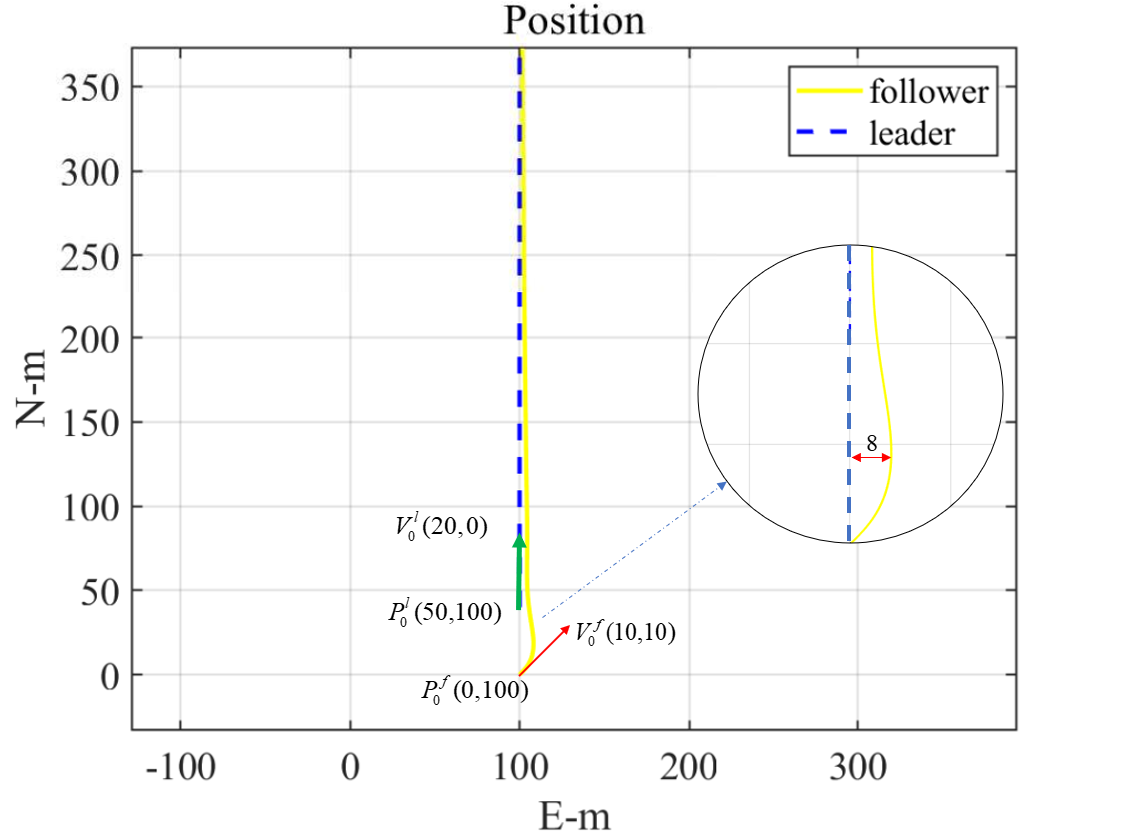
\includegraphics[width=0.85\textwidth]{figures/c5/c5-matlab-pos.png}
    \caption{水平面双机编队位置关系}\label{fig:c5-matlab-pos}
\end{figure}
\begin{figure}[H]
    \centering
    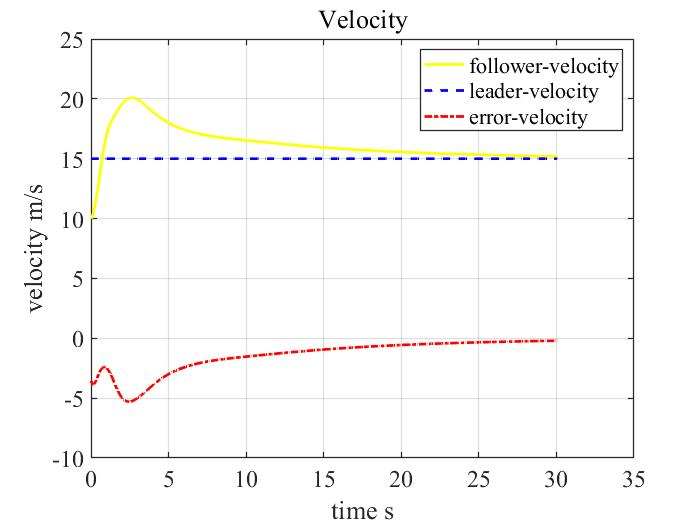
\includegraphics[width=0.85\textwidth]{figures/c5/c5-matlab-vel.jpg}
    \caption{水平面双机速度关系}\label{fig:c5-matlab-vel}
\end{figure}
\begin{figure}[H]
    \centering
    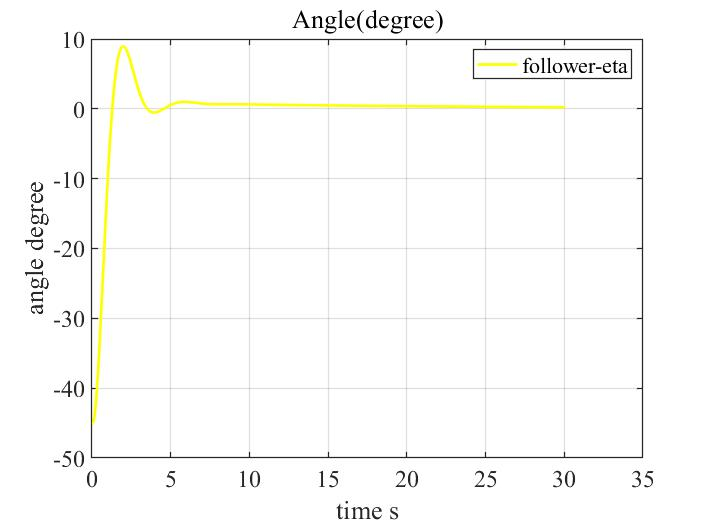
\includegraphics[width=0.85\textwidth]{figures/c5/c5-matlab-eta}
    \caption{水平面双机速度方向关系}\label{fig:c5-matlab-eta}
\end{figure}

竖直平面内,由于控制器的任务是消除高度误差以及追踪来自水平平面控制器的期望速度,控制量将是期望推力$T^{des}$以及期望俯仰角$\theta^{des}$,因而需要引入竖直平面内的无人机动力学模型(参见式\ref{point_dynamaic});按照之前的假设,无人机姿态内环为理想环节,可以用一个时间常数为$\tau_{\theta}$的惯性环节代替之。再结合式\ref{fol_motion_eauation},可以进行竖直平面的相关仿真:
为了方便读图,现在将$NED$坐标系下的$D$轴取反之后并用“$height$”表示:
从机的初始高度为:$h_0^{f}=10.0m$;
从机的初始速度大小为:$V_0^{f}=10.0m/s$;
从机期望高度为:$h^{des}=100.0m$
从机的期望速度为:$V^{des}=20.0m/s$
仿真的结果如下三图所示:
\begin{figure}[H]
    \centering
    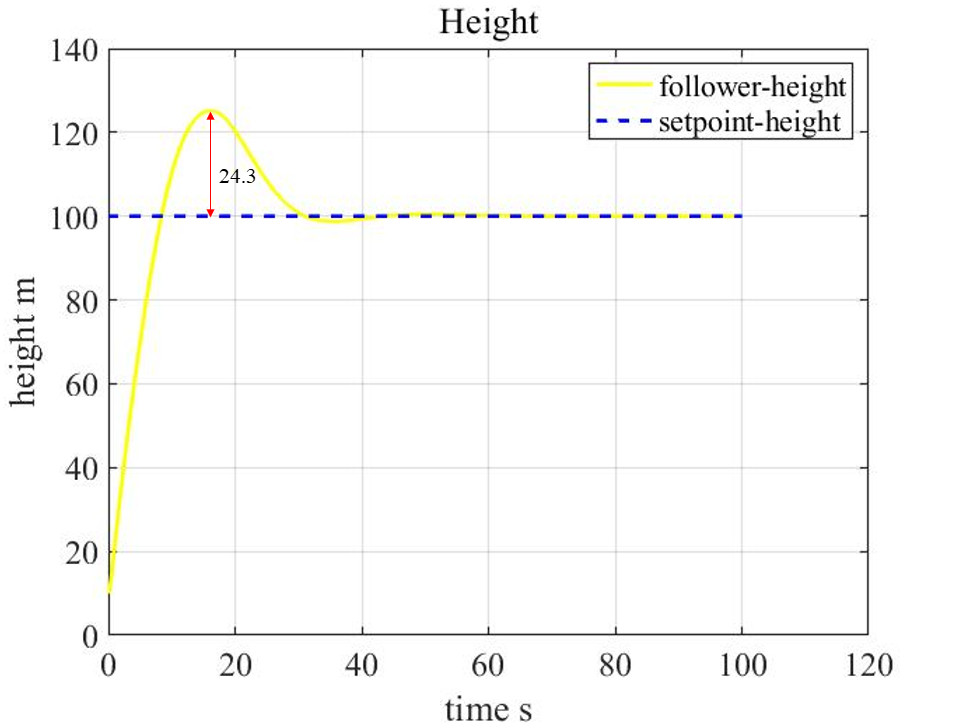
\includegraphics[width=0.85\textwidth]{figures/c5/c5-TECS-height.jpg}
    \caption{竖直平面高度关系}\label{fig:c5-TECS-height}
\end{figure}
\begin{figure}[H]
    \centering
    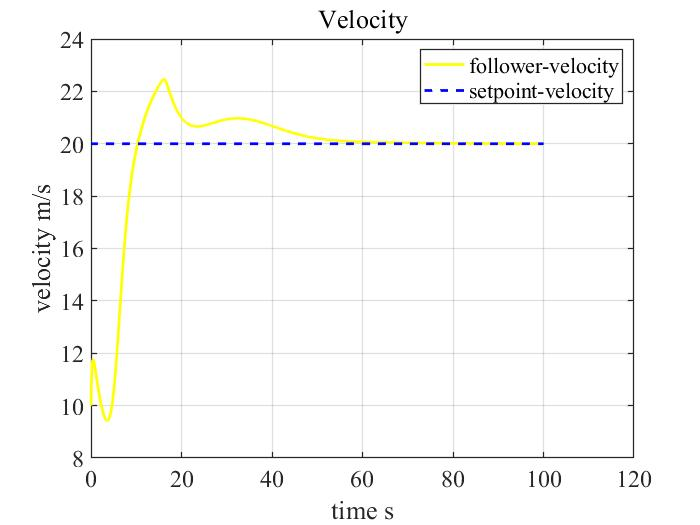
\includegraphics[width=0.85\textwidth]{figures/c5/c5-TECS-vel.jpg}
    \caption{竖直平面速度关系}\label{fig:c5-TECS-vel}
\end{figure}
\begin{figure}[H]
    \centering
    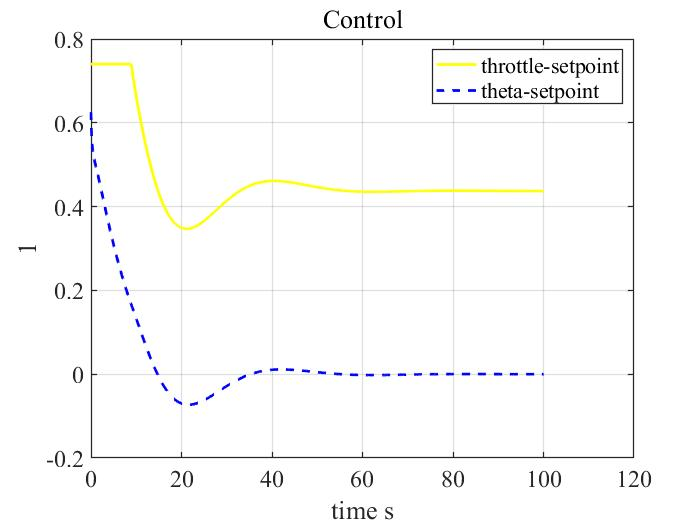
\includegraphics[width=0.85\textwidth]{figures/c5/c5-TECS-control.jpg}
    \caption{竖直平面控制量关系}\label{fig:c5-matlab-eta}
\end{figure}
由仿真结果可知,本文所设计的$TECS$控制器可以完成对于期望速度以及期望高度的跟踪,从而达到消除竖直平面内的误差的作用。
\section{基于ROS/Gazebo-PX4的双机编队动力学仿真}
